This section describes the Y layer in terms of its hardware and software design. The layer-level subsections below cover properties common to the whole layer (its Resource viewpoint); each subsystem is then described through the design viewpoints declared in Section 3. Include implementation specifics --- hardware components, programming languages, software dependencies, operating systems, data structures, and algorithms. Omit any viewpoint that does not apply (for example, a pure-software module has no hardware subsection). The organization and titles below may be adapted as necessary for the project.

\subsection{Layer Hardware}
Any hardware components common to the layer. For example, if each subsystem is a software process running on the same embedded computer, describe that device here. Do not list hardware that exists only at the subsystem level (cover it in the subsystem sections).

\subsection{Layer Operating System}
Any operating system(s) required by the layer.

\subsection{Layer Software Dependencies}
Any software dependencies (libraries, frameworks, runtimes) common to the layer.

\subsection{Subsystem 1}
Describe, at a high level, the purpose and basic design of this subsystem (its Context and Composition views): is it a piece of hardware, a class, a process, a web service, or something else, and what components make it up? The items below are specific to this subsystem, not a repeat of the layer-level material above.

\begin{figure}[h!]
	\centering
 	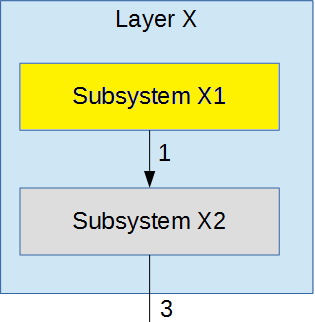
\includegraphics[width=0.60\textwidth]{images/subsystem}
 \caption{Example subsystem description diagram}
\end{figure}

\subsubsection{Subsystem Hardware}
\textit{(Resource viewpoint)} Any hardware components specific to this subsystem.

\subsubsection{Subsystem Operating System}
\textit{(Resource viewpoint)} Any operating system specific to this subsystem.

\subsubsection{Subsystem Software Dependencies}
\textit{(Resource viewpoint)} Any libraries, frameworks, or design tools specific to this subsystem.

\subsubsection{Subsystem Programming Languages}
\textit{(Resource viewpoint)} Any programming languages used by this subsystem.

\subsubsection{Subsystem Data Structures}
\textit{(Information viewpoint)} Any classes, records, schemas, or packet formats worth discussing. For example, data transmitted from a microcontroller to a PC over USB must be assembled into packets --- what is the packet structure?

\subsubsection{Subsystem Interfaces}
\textit{(Interface viewpoint)} The services, APIs, or signals this subsystem offers and requires. Use the interface identifiers established in the ADS so interfaces trace consistently across documents.

\begin {table}[H]
\caption {Subsystem 1 interfaces}
\begin{center}
    \begin{tabular}{ | p{1cm} | p{6cm} | p{3cm} | p{3cm} |}
    \hline
    ID & Description & Inputs & Outputs \\ \hline
    \#01 & Description of the interface/API/bus & \pbox{3cm}{input 1} & \pbox{3cm}{output 1}  \\ \hline
    \end{tabular}
\end{center}
\end{table}

\subsubsection{Subsystem Data Processing}
\textit{(Algorithm, Interaction \& State viewpoints)} The algorithms, control flow, and state behavior of the subsystem. If you implement a well-known algorithm, name it; if it is unique to this project, describe it in detail. Where behavior is stateful or sequenced, include a state or sequence diagram.

\subsubsection{Design Rationale}
Justify the key implementation choices for this subsystem (language, library, data structure, algorithm) against the alternatives, and reference the driving requirement IDs and any ADS architecture decisions.

\subsection{Subsystem 2}
Repeat for each subsystem in the layer.
